\documentclass[german, % Standardmäßig deutsche Eigenarten, englisch -> english
parskip=full, % Absätze durch Leerzeile trennen
bibliography=totoc, % Literatur im Inhaltsverzeichnis
%draft, % TODO: Entwurfsmodus -> entfernen für endgültige Version
]{scrartcl}
\usepackage{ifluatex} % zum Testen, ob LuaTeX verwendet wird
\ifluatex
\usepackage{fontspec} % Laden von Schriften
\setmainfont[Mapping=tex-text]{Linux Libertine O}  % Mapping ermöglicht die Verwendung z.B. von --
\setsansfont[Mapping=tex-text]{Linux Biolinum O}
\usepackage{polyglossia}  % Sprachpaket
\setdefaultlanguage[spelling=new,babelshorthands=true]{german}  % Neue Rechtschreibung und Abkürzungen
\else % kein LuaTeX
\usepackage[utf8]{inputenc} % Kodierung der Datei
\usepackage[T1]{fontenc} % Vollen Umfang der Schriftzeichen
\usepackage{lmodern}
\usepackage[ngerman]{babel} % Sprache auf Deutsch (neue Rechtschreibung)
%\usepackage{libertine} % Schriftart Linux Libertine/Biolinum verwenden
\fi

% Mathematik und Größen
\usepackage{amsmath}
\ifluatex
\usepackage{unicode-math}
\fi
\usepackage[locale=DE, % deutsche Eigenarten, englisch -> US
separate-uncertainty, % Unsicherheiten seperat
]{siunitx}
\usepackage{physics} % Erstellung von Gleichungen vereinfachen

% Bilder einbinden
\usepackage{graphicx}
\usepackage{float}
\usepackage{caption}
%\graphicspath{{bilder/}} % TODO: Pfad unter dem die Bilder gesucht werden

% Gestaltung
\usepackage{microtype}  % Mikrotypographie
\usepackage{booktabs}  %schönere Tabellen
\usepackage[toc]{multitoc}  %mehrspaltiges Inhaltsverzeichnis
\usepackage{csquotes} % Anführungszeichen mit \enquote
\usepackage{subcaption}  % Unterabbildungen a,b,c,…
\usepackage{enumitem}  % Listen anpassen
\setlist{itemsep=-10pt}
\usepackage{scrpage2}  % Manipulation des Seitenstils
% Kopf-/Fußzeilen
\pagestyle{scrheadings}
\clearscrheadings
\automark{section}
\ofoot{\pagemark}
\ihead{\headmark}
\setheadsepline{.5pt}

\usepackage[colorlinks=true]{hyperref}  % Links und weitere PDF-Features

\makeatletter 
\renewcommand\subsection{\@startsection 
   {subsection}{2}{0mm}%      % name, ebene, einzug 
   {0.5\baselineskip}%            % vor-abstand 
   {0.3\baselineskip}%            % nach-abstand 
   {\bfseries\sffamily\large}%           % layout 
   } 
\makeatother 

% TODO: Titel und Autor, … festlegen
\newcommand*{\titel}{Optische Kohärenztomographie}
\newcommand*{\autor}{Maximilian Obst, Thomas Adlmaier}
\newcommand*{\abk}{OCT}
\newcommand*{\betreuer}{M.Sc. Jonas Golde}
\newcommand*{\messung}{28.10.2016}
\newcommand*{\ort}{Medizinische Fakultät Carl Gustav Carus}

\hypersetup{pdfauthor={\autor}, pdftitle={\titel}} % PDF-Metadaten

\titlehead{F-Praktikum \abk \hfill TU Dresden}
\subject{Versuchsprotokoll}
\title{\titel}
\author{\autor}
\date{\begin{tabular}{ll}
Protokoll: & \today\\
Messung: & \messung\\
Ort: & \ort\\
Betreuer: & \betreuer\end{tabular}}

%----------------
\begin{document}
\begin{titlepage}
\maketitle

\begin{figure}[hb] 
  \centering
     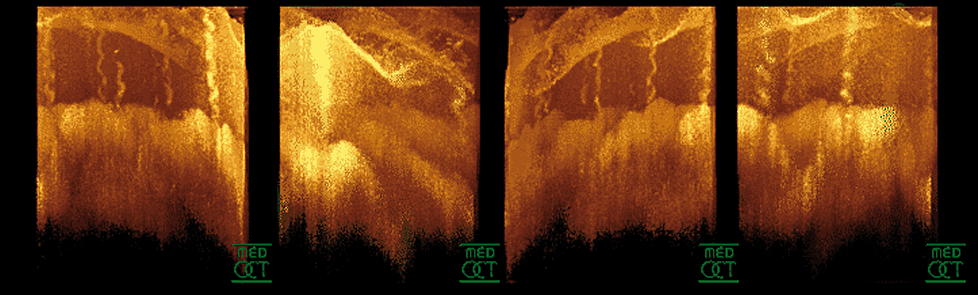
\includegraphics[width=0.7\textwidth]{tomographie}
  \caption{Fingerkuppe unter optische Kohärenztomographie	\cite{bild-tomographie}}
  \label{fig:tomographie}
\end{figure}
\end{titlepage}

\tableofcontents
\pagebreak

%------------------------
\section{Physikalische Grundlagen}

Die Optische Kohärenztomographie ist ein bildgebendes Verfahren, welches vor allem in der Humanmedizin verwendet wird. Dort schließt es die Lücke zwischen Sonographie, welche sehr tief in den Körper eindringen kann, aber nur eine grobe Auflösung bietet, und Mikrokopie, die nur die Oberfläche abbilden kann. Die optische Kohärenztomographie bildet die ersten Millimeter des Gewebes mit hoher Auflösung ab.
In diesem Versuch wird eine Einführung in die Arbeit mit OCT geboten. Es wird sowohl Time Domain OCT als auch Frequency Domain OCT durchgeführt.

\subsection{Einführung}

Bei der Optischen Tomographie wird ein Material mit Licht einer bestimmten Wellenlänge im Infrarotbereich beschienen. Besonders eignen sich die Wellenlängen um 800\,nm, die eine besonders gute Auflösung der Bilder liefern, und die Wellenlängen um 1300\,nm, welche besonders tief in menschliches Gewebe eindringen können. Das vom Gewebe reflektierte Licht wird in einem Michelson-Interferometer mit dem von einem Referenzarm reflektierten Licht überlagert. Aus dem Interferenzbild kann ein räumliches Bild des Materials gewonnen werden. 

\subsection{Time Domain OCT}

Bei der Time Domain OCT (TD OCT) wird breitbandiges, kurzkohärentes Licht verwendet. Damit wird gewährleistet, dass Interferenz nur entsteht, wenn beide Arme annähernd gleich lang sind. Die Kohärenzlänge bestimmt damit direkt die axiale Auflösung. Durch Verschiebung des Referenzspiegels, sodass die Interferenz bestehen bleibt, kann die Tiefe der Reflexion bestimmt werden. Durch die nötige mechanische Arbeit können nur Wiederholungsraten von wenigen kHz erzeugt werden. Aufgezeichnet wird nur die Intensität der Interferenz.\\
Die normierte komplexe Selbstkohärenzfunktion stellt den Interferenzterm da: 
\begin{align}
\gamma ( \tau ) = e^{-i \Omega \tau} e^{\frac{1}{16 \ln 2} ( \Delta \Omega \tau )^2} 
\end{align}
\begin{align*}
\Omega = \text{Kreisfrequenz;} \ \tau = \text{Laufzeitdifferenz}
\end{align*}
Kohärenzlänge und axiale Auflösung: 
\begin{align}
l_c = \frac{2 \ln 2}{\pi} \frac{\lambda_c^2}{\Delta \lambda} 
\end{align}
\begin{align*}
\lambda_c = \text{Zentralwellenlänge des Laserspektrums}
\end{align*}

\subsection{Frequency Domain OCT}

Bei der Frequency Domain OCT (oder auch Fourier Domain OCT; FD OCT) wird im Unterschied zur TD OCT nicht nur die Intensität des Interferenzsignals, sondern des ganzen Interferenzspektrum aufgezeichnet, indem das Licht spektral zerlegt wird. Damit kann die gesamte Tiefeninformation gleichzeitig aufgenommen werden und das Signal-Rausch-Verhältnis ist wesentlich besser. Es gibt zwei Varianten: Die Spectral Domain OCT (SD OCT), bei der das Licht durch ein Spektrometer gefiltert wird, und die Swept Source OCT (SS OCT), bei der die Wellenlänge des Lichts durchgestimmt wird. Die Wiederholungsrate wird bei SD OCT durch die Auslesegeschwindigkeit der Fotochips bestimmt und liegt bei etwa 200\,kHz. \\
Axiale Auflösung:
\begin{align}
FWHM_z = \frac{\sqrt{2 \ln 2}}{n}\frac{\lambda_c^2}{2 \pi \sigma_\lambda} = \frac{2 \ln 2}{\pi n}\frac{\lambda_c^2}{FWHM_\lambda} 
\end{align}
\begin{align*}
\sigma_\lambda = \text{Standardabweichung bezüglich der Wellenlänge;} \ n = \text{Brechungsindex der Probe;} \\ FWHM_\lambda = \text{Halbwertsbreite des Laserspektrums}
\end{align*}
Maximale Eindringtiefe:
\begin{align}
z_{max} = \frac{\pi}{2 \delta k} = \frac{\lambda_c^2}{4 \delta \lambda}
\end{align}

\subsection{Doppler FD OCT}

Mit Hilfe der Doppler FD OCT können schließlich auch Geschwindigkeiten quantitativ untersucht werden. Dafür muss nun neben der Intensität auch die Phase $\phi$ mit aufgenommen werden. Eine aufgenommene Phasenverschiebung deutet eine axiale Verschiebung an, also eine Geschwindigkeit des untersuchten Materials.
\begin{align}
\Delta \phi = 2 k \Delta z_s
\end{align}
Berechnet werden kann die Geschwindigkeit dann anhand dieser Formel:
\begin{align}
v(z) = \frac{\lambda_0 \phi (z)}{4 \pi n T_{A-Scan} \sin (\theta)}
\end{align}
Problematisch ist dabei der endliche Strahldurchmesser $\omega_0$, der zu einer Wichtung der aufgenommenen Amplituden und Phasen führt. Um mit dieser Wichtung umzugehen, werden zunächst dimensionslose Größen eingeführt:
\begin{align}
\delta x = \frac{\Delta x}{\omega _0}
\end{align}
Solange $\delta x$ kleiner als 1 ist, beschreibt das klassische Dopplermodell das Problem hinreichend.

\subsection{Signalverarbeitung}

Um die Signale aus dem OCT zu verarbeiten, müssen verschiedene Umformungen vorgenommen werden: Zunächst muss ein Dechirp vorgenommen werden, der Verzerrungen ausgleicht, indem er reskaliert. Dann wird über das Spektrum ein Hanning-Fenster gelegt. Dieses schwächt das Rauschen ab, führt aber zu einer Auflösungsverschlechterung. Schließlich wird mit Fast Fourier Transformation das Tiefenprofil erstellt. Die Intensitätsdarstellung wird dabei in die logarithmische Skala überführt und als 8\,bit Grauwert ausgegeben.

\section{Durchführung}

Der Versuch wird mit einem FD OCT-Gerät durchgeführt. Die verwendete Zentralwellenlänge $\lambda_0$ beträgt $845\,nm$ bei einer Bandbreite von $\Delta \lambda = 35\,nm$. Das Auslesen erfolgt mit einer Geschwindigkeit von $11888,2\,Hz$.

\subsection{Time Domain OCT}

Zunächst soll TD OCT durchgeführt werden. Da das Gerät selbst auf FD OCT beruht, muss die TD OCT simuliert werden. Dafür wird auf einem Lautsprecher ein Spiegel angebracht. Somit tauschen der Referenzarm und der Probenarm ihre Funktion. Um die Messung durchzuführen, muss zunächst der Spiegel fokussiert werden. Dann wird der Lautsprecher bei einer Frequenz von $20\,Hz$ zum Schwingen gebracht. Die Aufnahme erfolgt mit dem Programm TD\_OCT.vi. Die Messdaten werden gespeichert.

Um die Geschwindigkeit des Lautsprechers zu bestimmen, muss danach noch mit FD OCT die Amplitude der Schwingung gemessen werden. Dafür wird das Programm \\ OCT\_MAXIMUS\_Doppler.vi verwendet und die aufgenommenen Messdaten wieder gespeichert. 

\subsection{Frequency Domain OCT}

Hier soll zunächst die axiale Auflösung des Geräts untersucht werden. Dafür wird eine aufgeraute, $5\,mm$ dicke Glasplatte in den Strahlengang gehalten und fokussiert, sodass der Oberflächenreflex gut zu sehen ist. Die Daten werden gespeichert.

Als nächstes wird eine medizinische Messung durchgeführt. Dafür werden zwei Finger in den Strahlengang gehalten und fokussiert: Ein eingecremter Finger und ein uneingecremter. Nach der Messung an jeweils drei Stellen der Finger werden beide für 10 Minuten in ein Wasserbad gehalten. Dann wird an den selben Stellen wieder ein Bild aufgenommen. Dies wird nach nochmals 10 Minuten im Wasserbad wiederholt.

\subsection{Doppler FD OCT}

Als letztes soll in einer runden Glaskapillare mit einem Innendurchmesser von etwa $300\, \mu m$ die Fließgeschwindigkeit quantitativ bestimmt werden. Dafür wird eine Lösung aus $2\,ml$ Intralipid20 und $48\,ml$ destilliertem Wasser hergestellt. Dann wird der tatsächliche Innendurchmesser an der untersuchten Stelle gemessen, indem dort ein Bild der leeren Kapillare nach der Fokussierung aufgenommen wird. Dann wird zur Bestimmung des Brechungsindex der Kapillare ein Bild der mit der Lösung durchsetzten Kapillare gemacht. 

Zur Bestimmung der Fließgeschwindigkeit muss zunächst der korrekte Dopllerwinkel eingestellt werden. Danach wird ein Volumenstrom eingestellt, der zu einer maximalen Fließgeschwindigkeit unterhalb der Schwelle zum erweiterten Dopllermodell führt. Schließlich werden mit dem Programm OCT\_MAXIMUS\_Doppler.vi die Geschwindigkeitsprofile aufgenommen und gespeichert. 

\section{Analyse}

\subsection{Time Domain OCT}

\begin{figure}[ht]
	\centering
	\begin{subfigure}[b]{0.4\textwidth}
	   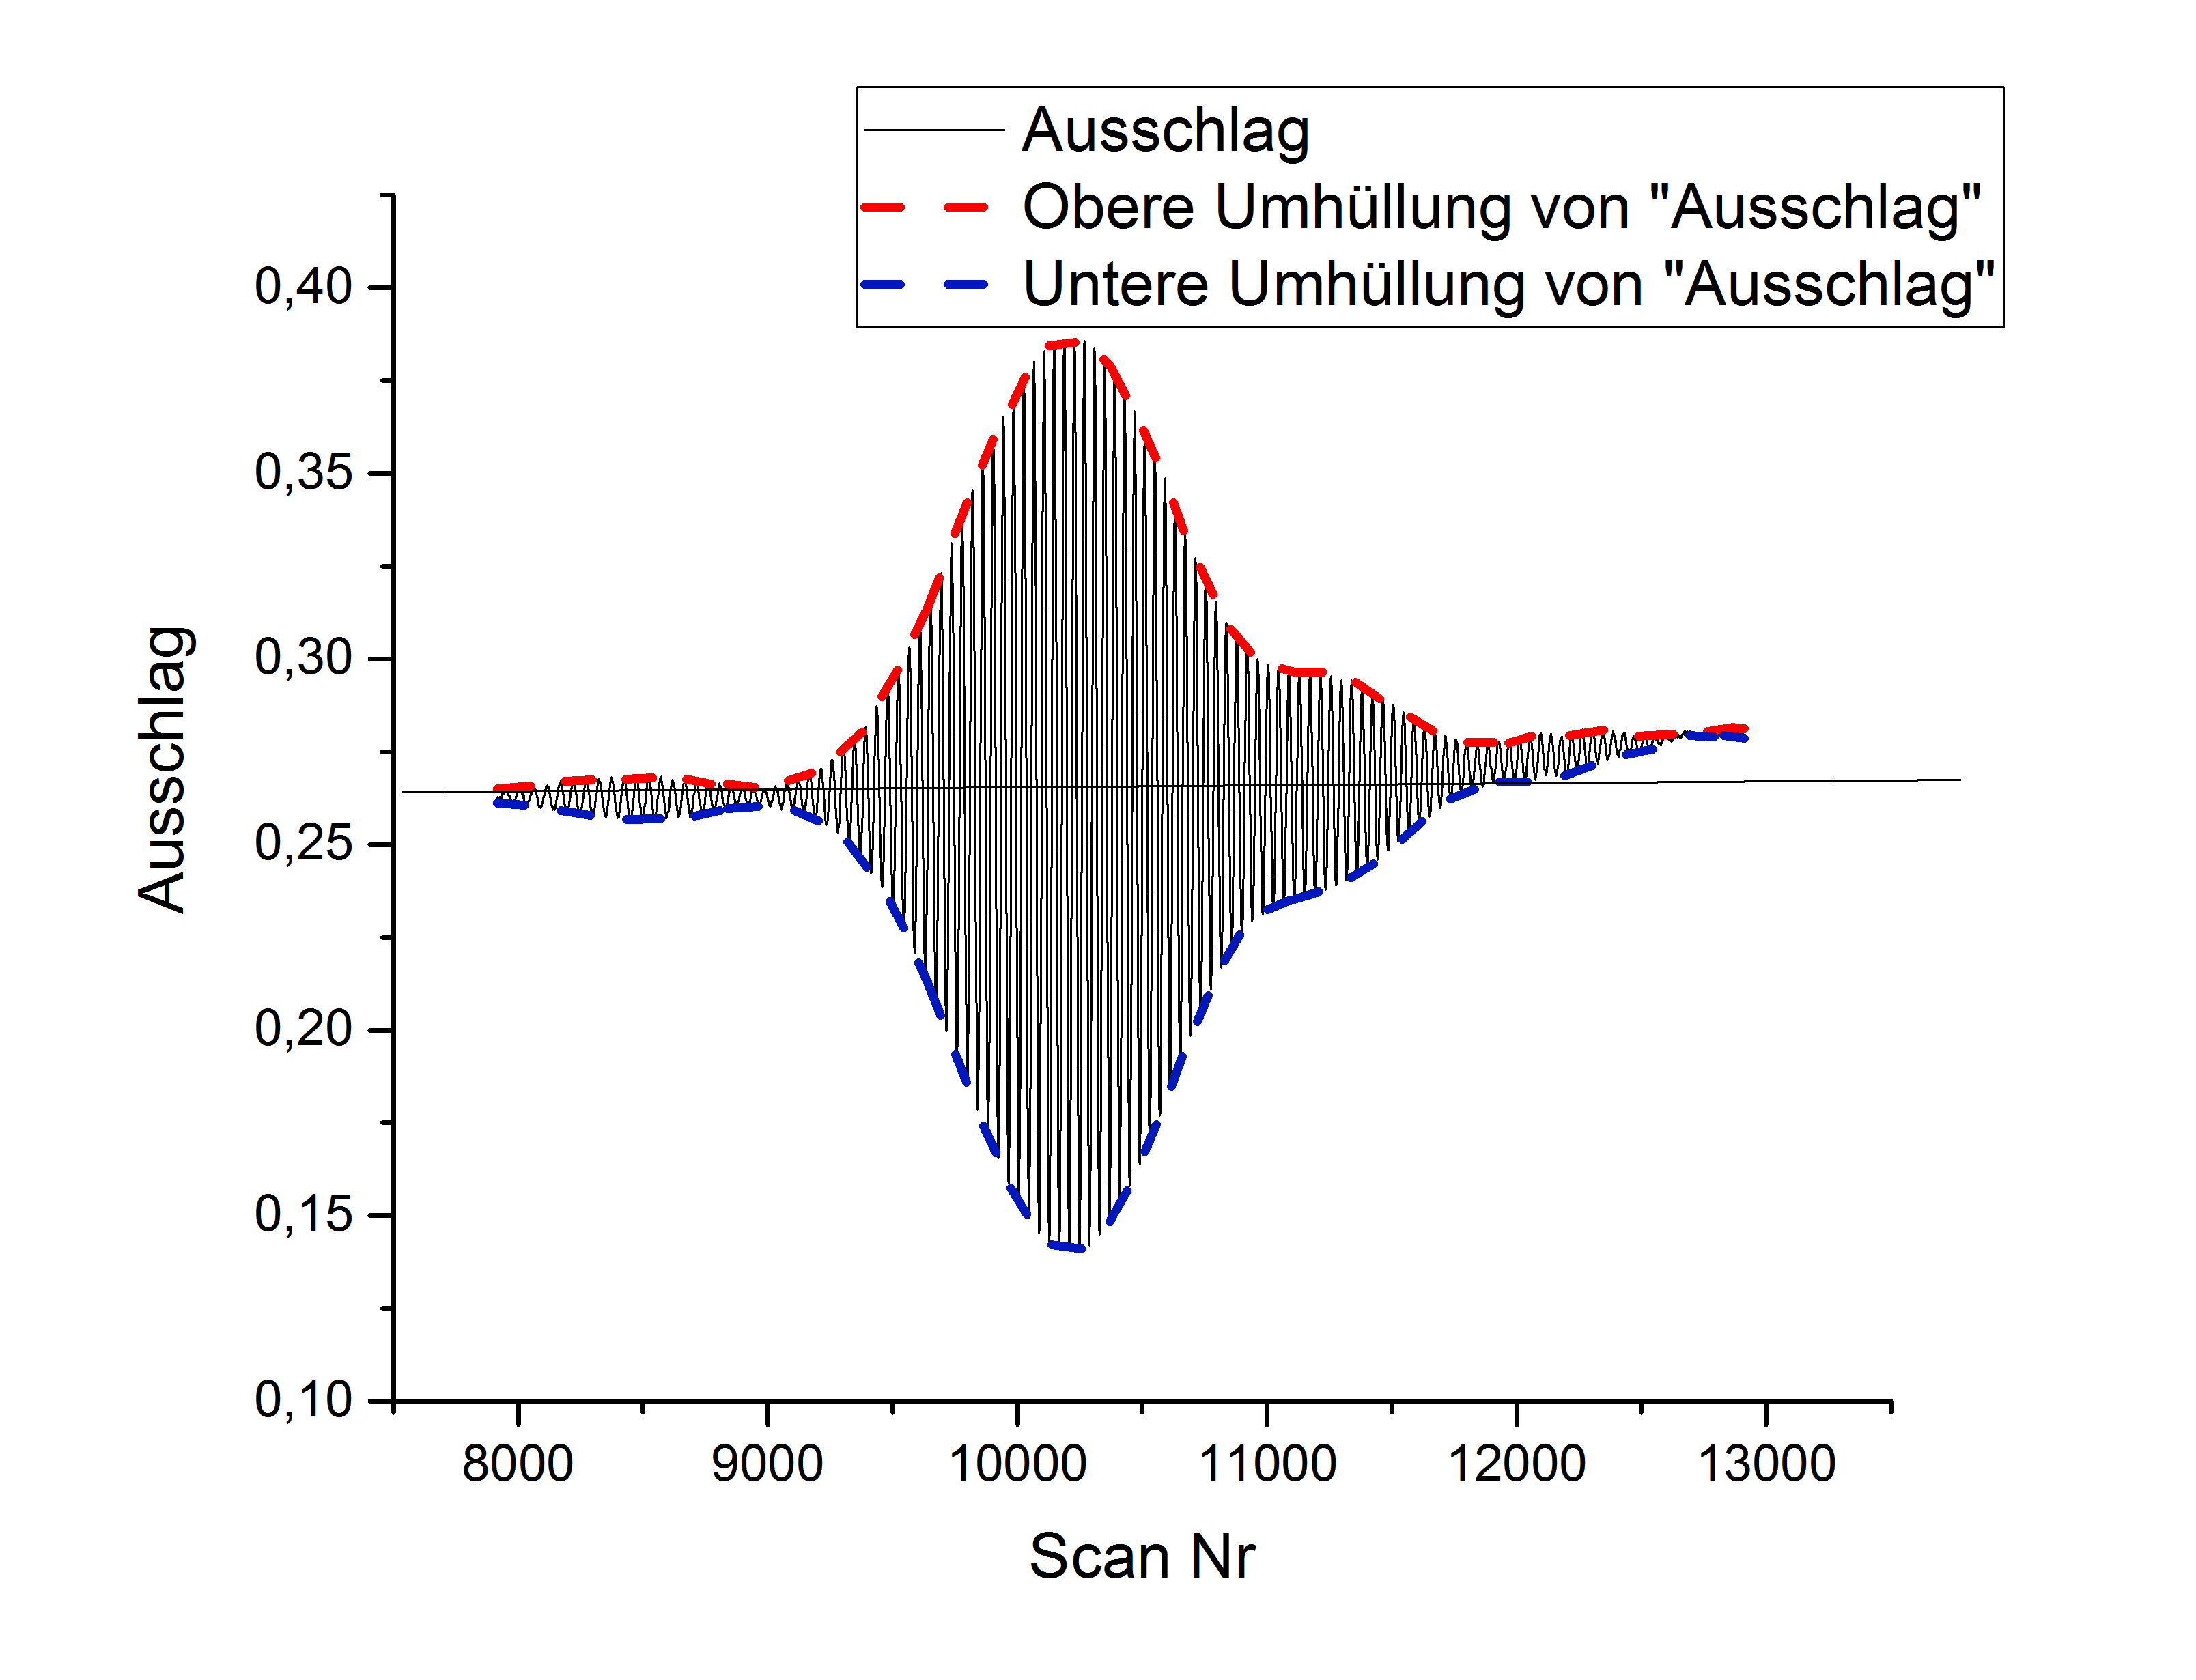
\includegraphics[width=\textwidth]{TD_OCT_DATA_Einhullende}
		 \caption{Mit TD OCT gemessene Ausschlagsfunktion des Lautsprechers}
	\end{subfigure}
	\begin{subfigure}[b]{0.4\textwidth}
	   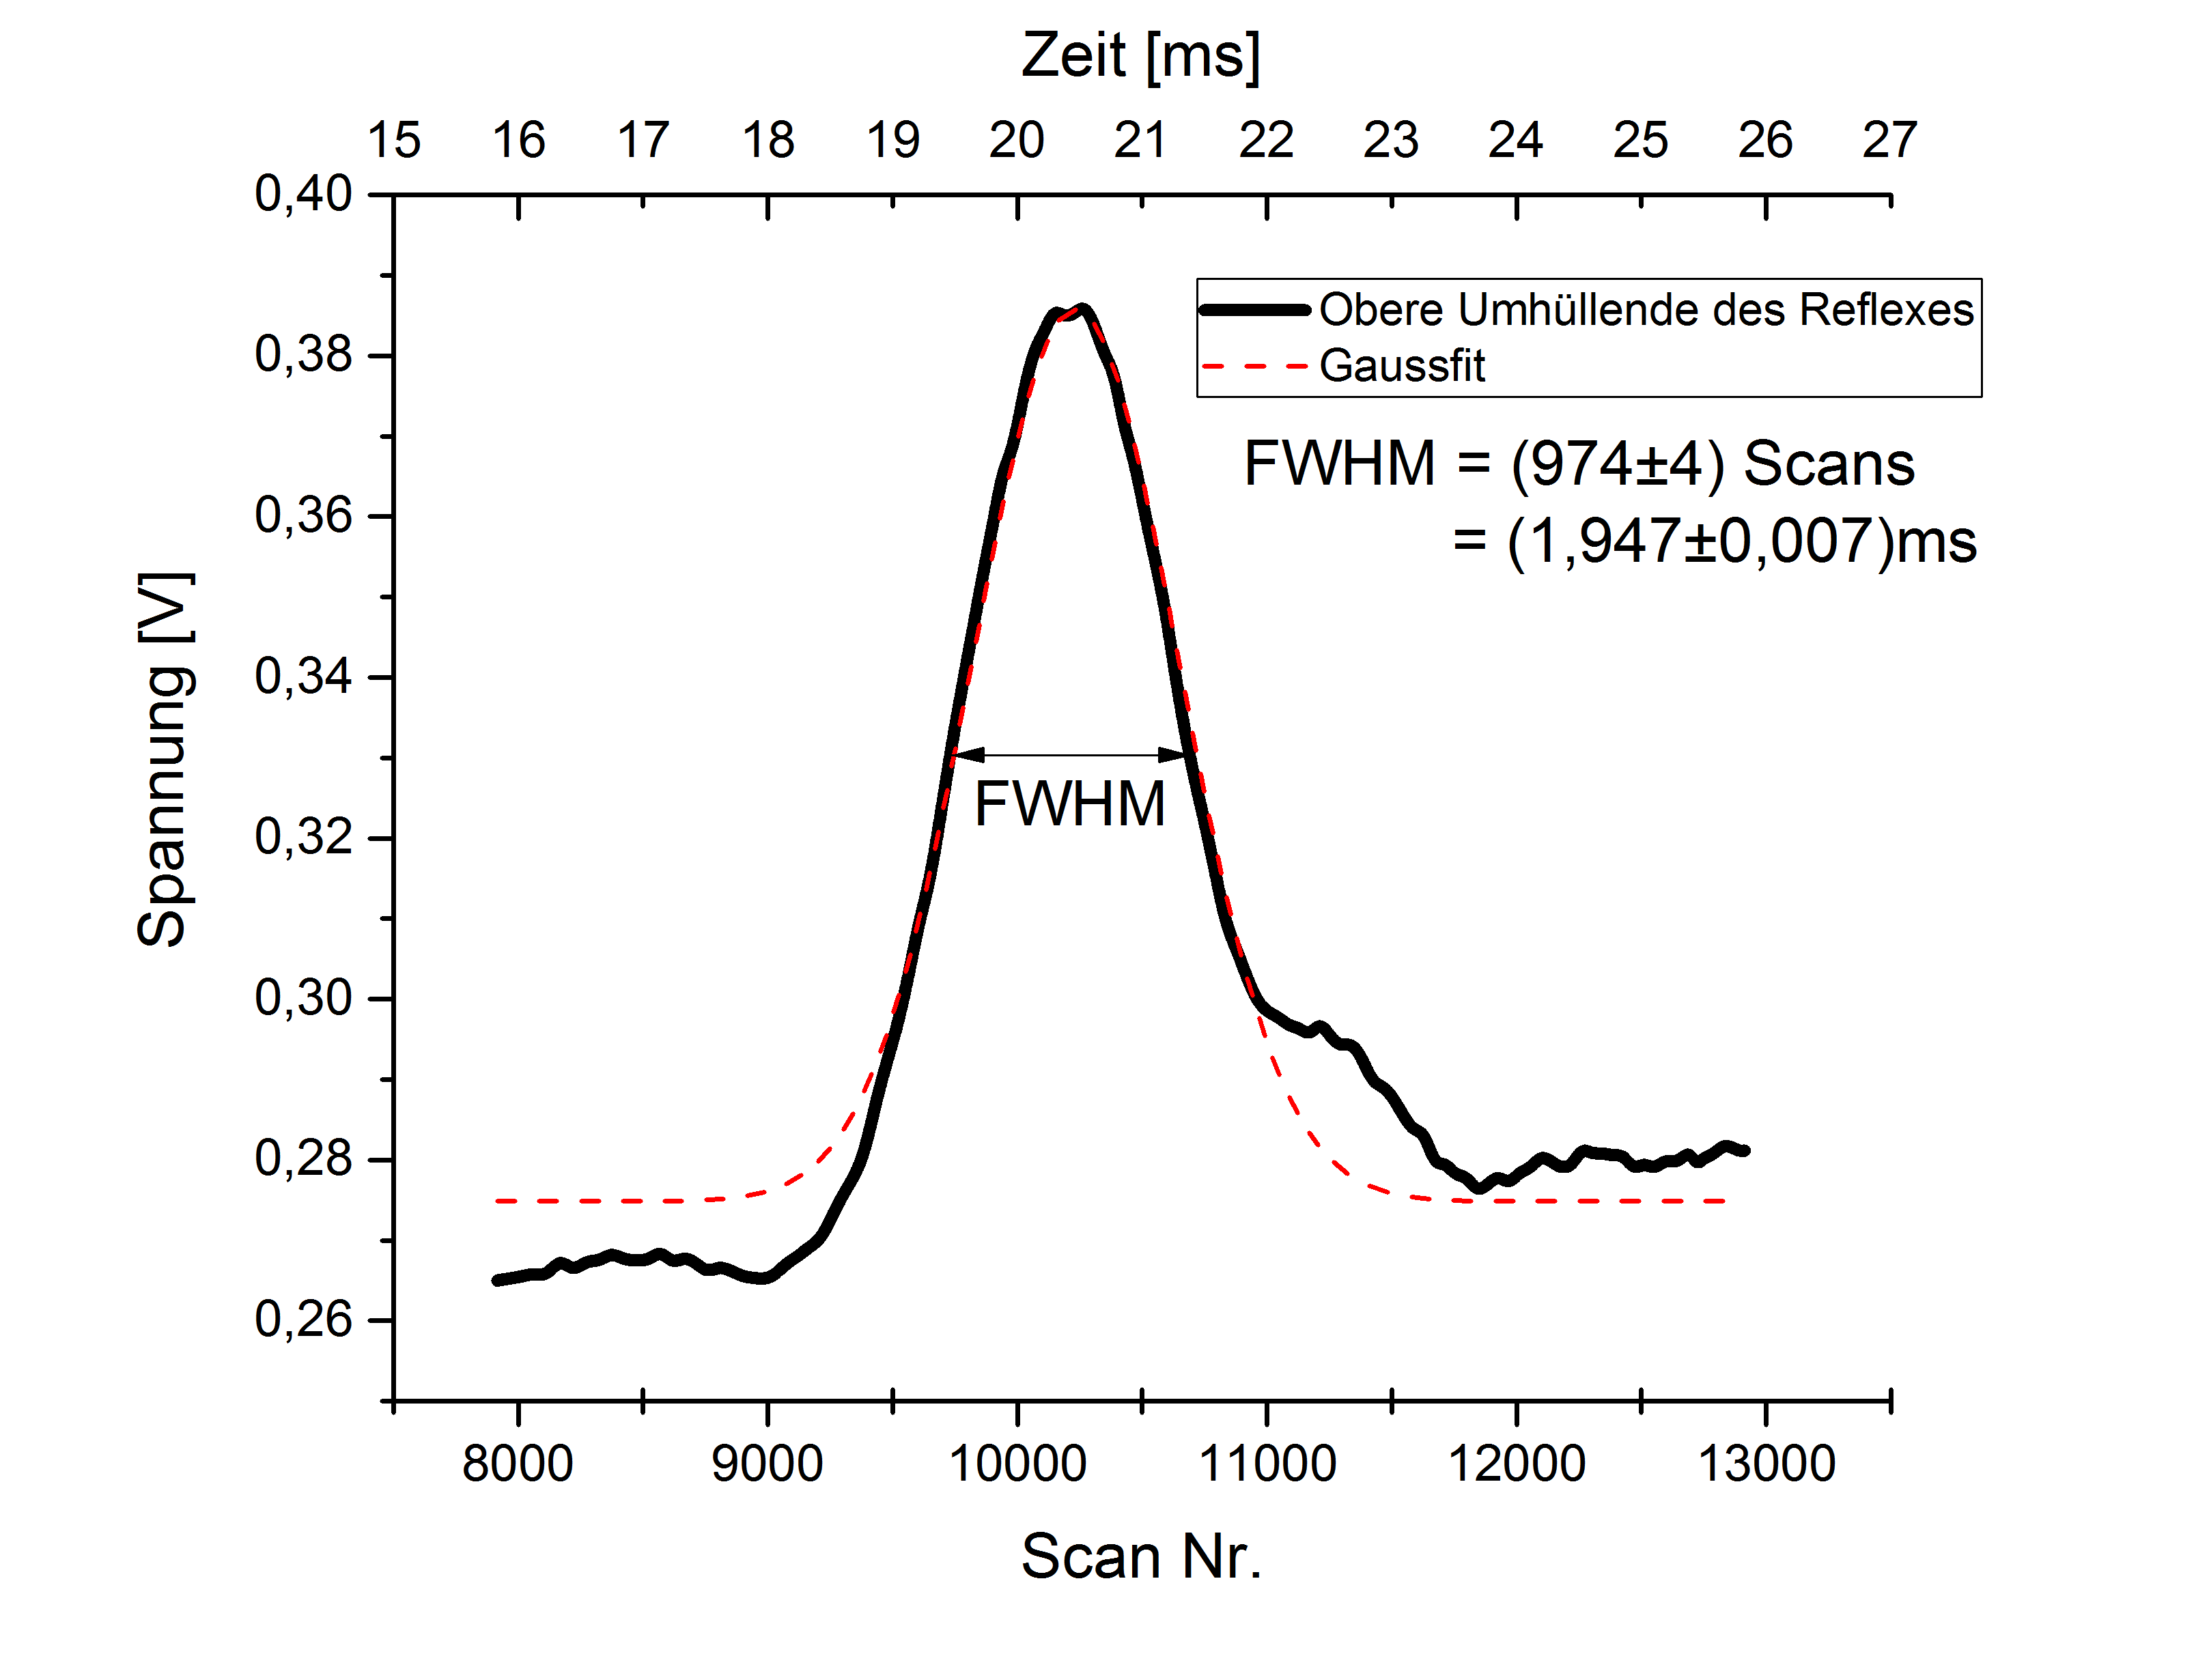
\includegraphics[width=\textwidth]{TD_OCT_FINAL}
		 \caption{Berechnete Einhüllende der Funktion}
	\end{subfigure}
  \caption{Einhüllende des Ausschlags}
	\label{fig:hull}
\end{figure}

Die Frequenzfunktion wird mit der simulierten TD OCT aufgenommen. Aus der Einhüllenden, die in Bild \ref{fig:hull} zu sehen ist, wird die Schwingungsdauer ermittelt:
\begin{align*}
T_{Schwingung} = (0.0253 \pm 0.0007) s
\end{align*}

\begin{figure}[hb] 
  \centering
     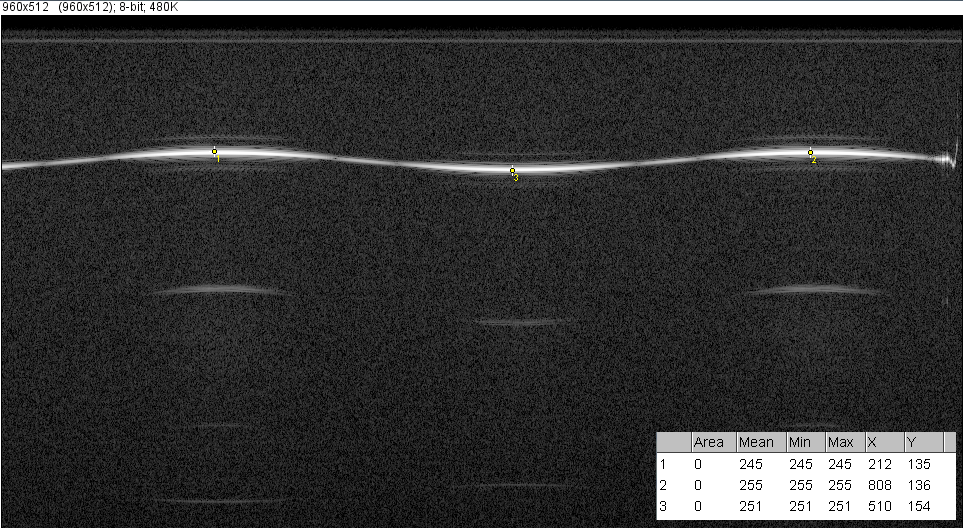
\includegraphics[width=0.7\textwidth]{Amplitude_Beispiel}
  \caption{Auswertung der aufgenommenen Schwingungsamplitude des Lautsprechers}
  \label{fig:amplitude}
\end{figure}

Die Schwingungsamplitude wird mit FD OCT aufgenommen. Das enstandene Bild kann in Bild \ref{fig:amplitude} gesehen werden.
\begin{align*}
l_{Amplitude} = (49 \pm 4) \mu m
\end{align*}

Die experimentelle Auflösung wird aus der Geschwindigkeit des Lautsprechers bestimmt:
\begin{align}
l_{c; exp.} = ???
\end{align}
Diese wird aus der gemessenen Schwingungsdauer und Amplitude ermittelt, der Fehler wird über die Gauss'sche Fehlerfortpflanzung bestimmt:
\begin{align}
v_{Lautsprecher} = \frac{2l_{Amplitude}}{T_{Schwingung}} \\
\Delta v_{Lautsprecher} = \sqrt{\left( \frac{2 \Delta l_{Amplitude}}{T_{Schwingung}} \right)^2 + \left(-\frac{2l_{Amplitude} \Delta T_{Schwingung}}{T_{Schwingung}^2} \right)^2}
\end{align}

Die theoretische Auflösung der TD OCT wird mit der Formel 2 berechnet. 
\begin{align*}
l_{c; th.} = 9.0022 \mu m
\end{align*}

\subsection{Frequency Domain OCT}

\begin{figure}[ht] 
  \centering
     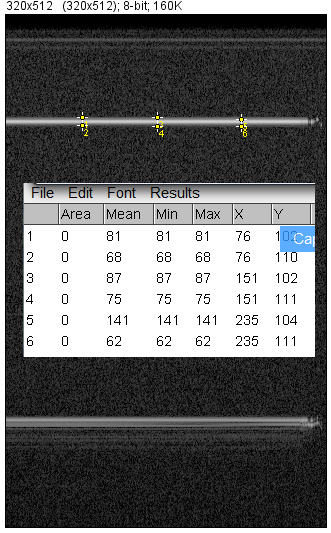
\includegraphics[width=0.7\textwidth]{Glasplatte_Auswertung}
  \caption{Auswertung des aufgenommenen Bildes der Glasplatte}
  \label{fig:glasplatte}
\end{figure}



\section{Fazit}

%------------------------

\begin{thebibliography}{9}

\bibitem{bild-tomographie}
  http://www.zwp-online.info/sites/default/files/users/kerstin/kohaerenz3.png

\end{thebibliography}

\end{document}
